%\documentclass{article}
\documentclass[a4paper,10pt]{article}
\usepackage[utf8]{inputenc}
\usepackage{graphicx}
\usepackage{url}
\usepackage{float}
\usepackage{times}
\usepackage{multirow}
\usepackage{listings}
\usepackage{times}
\usepackage{paralist}
\usepackage{epsfig}
\usepackage{subfigure}
\usepackage[hypertex]{hyperref}
\usepackage{subfigure}
\usepackage{color}

%\documentclass{rspublic}

\usepackage{ifpdf}

\newcommand{\I}[1]{\textit{#1}}
\newcommand{\B}[1]{\textbf{#1}}
\newcommand{\BI}[1]{\textbf{\textit{#1}}}
\newcommand{\T}[1]{\texttt{#1}}

\pdfpagewidth 8.5in
\pdfpageheight 11in 

\setlength\topmargin{0in}
\setlength\headheight{0in}
\setlength\headsep{0in}
\setlength\textheight{9in}
\setlength\textwidth{6.5in}
\setlength\oddsidemargin{0in}
\setlength\evensidemargin{0in}
\setlength\parindent{0.1in}
\setlength\parskip{0.25em}

\ifpdf
 \DeclareGraphicsExtensions{.pdf, .jpg}
\else
 \DeclareGraphicsExtensions{.eps, .ps}
\fi

\newcommand{\jha}[1]{ {\textcolor{red} { ***Jha: #1 }}}

\begin{document}

\title{\large Implementing Abstractions for Data Intensive Applications using SAGA}

\author{Shantenu Jha$^{1,2}$, Hartmut Kaiser$^{1}$, Michael Miceli$^{1}$, Christopher Miceli$^{1}$, \\ Joao Abecasis$^{1}$\\
  \small{\emph{$^{1}$Center for Computation \& Technology, Louisiana State University, USA}}\\
  \small{\emph{$^{2}$Department of Computer Science, Louisiana State
      University, USA}}}

\maketitle


The deluge of data is upon us and there exist a critical need to be
able to access, manage and mine this data. There is a need for
abstractions to support data-intensive computing, and these
abstractions are required at several levels -- programmatic, system
and data-access patterns.

For example, the power of Google is based upon a simple programming
abstraction -- MapReduce~\cite{mapreduce}.  MapReduce is a framework
for splitting up large data and keeping track of which machine the
data is on. The purpose is to automatically parallelize and execute on
large clusters.  The application itself has to provide only the
specific map and reduce steps, reusing the bulk of the functionality
from the provided generic implementation.  By relieving the
end-developer from having to control explicitly data placement, job
distribution, load balancing, etc., MapReduce provides a level of
abstraction that simplifies the task of an application programmer.

There exist additional powerful abstractions, such as
AllPairs~\cite{allpairs}, which is both a programming abstractions and
a system-level abstraction.  Allpairs is a framework for when every
element of some data needs every other element of another set of data.
When implemented on distributed infrastructure, AllPairs, like
MapReduce, essentially decouples the client's code from grid specific
information.  Again, all the application has to provide is the
ordering criteria of the data to work on, resuing the programming
abstractions as implemented by the based framework.

% Many similar problems arise, when designing distributed applications.
% If there is a level of abstraction between the user and the
% grid-specific problems then designing applications become much
% simpler. 

SAGA~\cite{saga_gfd90} is a high level API that provides a simple,
standard and uniform interface to the most commonly required
distributed functionality.  SAGA can be used to encode grid
applications~\cite{saga_escience07, saga_tg08}, tool-kits to manage
distributed applications as well as implement abstractions that
support commonly occurring programming, access and usage patterns.
The focus of this paper is on the latter set, i.e.  the use of SAGA in
implementing well known abstractions for data intensive computing.

In this paper, we will implement MapReduce and All-Pairs abstractions
using SAGA and use them to solve commonly encountered genomic tasks.
We will show how multiple sequence alignment can be orchestrated using
the SAGA-Allpair implementation, and genome searching can be
implemented using Map-reduce.  In addition, the aim of this paper is
to show (validate) that SAGA is a sufficiently complete and high-level
interface so as to support these programming abstractions.

% This paper will focus on how to create a useful and efficient
% implementation of both MapReduce and AllPairs using SAGA.  

Figure~\ref{fig:data_intensive_app_saga} illustrates the software
architecture of the implementation, highlighting the different
abstraction levels that allow the reuse of most of the system for both
algorithms and for different genomic applications.  We will highlight
the sailent points of our implementations, and how we handle common
considerations such as when to move the data to the machine or when to
process it locally.  The implemention of these abstractions
encapsulates details such as latency hiding, performance and other
variables (such as cluster sizes, and queue sizes).  The user should
be able to easily add a few function calls without worrying about many
considerations required by most grid computing applications.

We will discuss other performance issues that arise when implementing
abstractions specific for data-intensive computing.  A grid
application's design should not focus on the bandwidth of the network,
the dispatch latency, the number of machines available, and data
reliability.  Even something as simple as process size can be a tough
challenge to optimize.  If a job is too small, then network traffic
becomes a bottleneck and the design is inefficient.  If a job is too
large, it is difficult to tell when it is hanging or still computing.
Also, if another job with a higher priority takes a machine over, the
application will be waiting on jobs longer.  The main point of this
paper is to show how a flexible, extensible implementation of
programming data-intensive abstractions using SAGA can shield the
application developer many of these considerations.



%these that can serve as a basis for data intensive applications.

% the mapreduce framework as well as a good guide for parallel
% programming.

\begin{figure}
\begin{center}
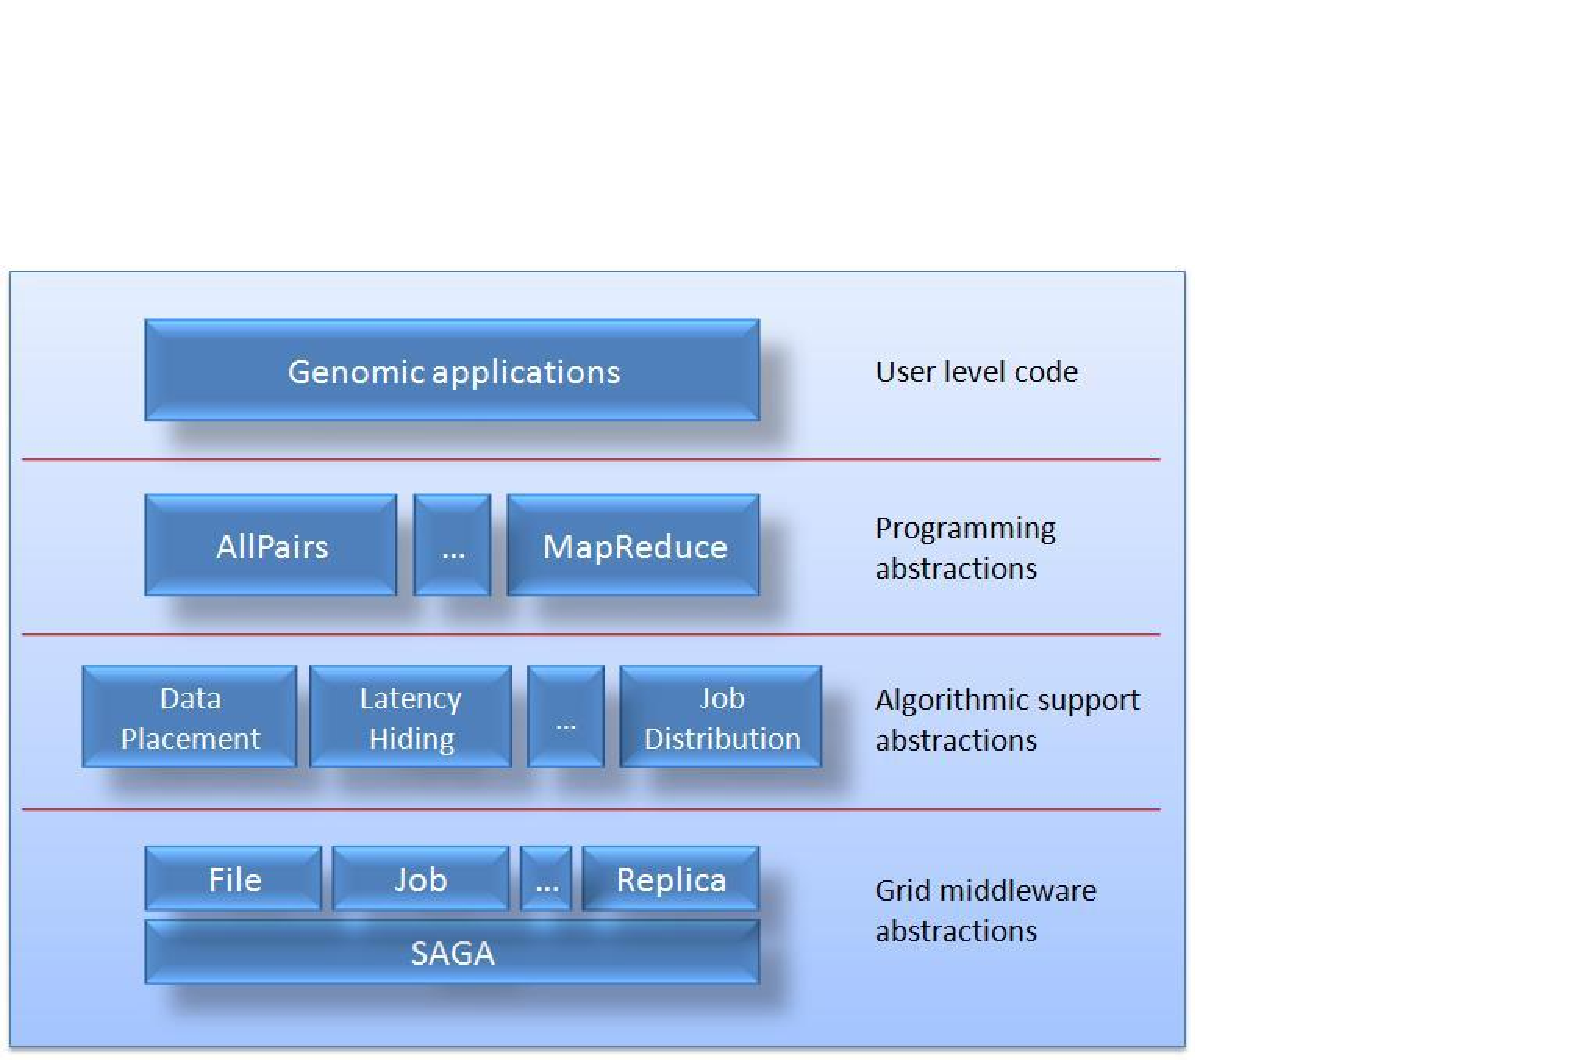
\includegraphics[scale=0.60]{data_intensive_app_saga}
\end{center}
\caption{The programming abstractions provided by the AllPairs and
  MapReduce algorithm implementations are sufficient to enable a wide
  range of genomic aplications (sequence alignment, searching, etc.)
  to be distributed over grids. The required underlying functionality
  is provided by higher level algorithmic support abstractions, such
  as tools for data placement, latency hiding, and job distribution,
  which ar ebeing built on top of grid middleware abstractions
  provided by SAGA (such as file transfer, job launching, information
  services and replica management.}
\label{fig:data_intensive_app_saga}
\end{figure}

\bibliographystyle{IEEEtran} 
\bibliography{saga}
\end{document}



% Distributed mergesort is an important example that can be used in many
% distributed applications. \ It encompasses all 4 phases of designing a
% successful parallel algorithm: \ partitioning, communication,
% agglomeration, and mapping. \ By designing and implementing a flexible
% implementation of distributed mergesort, different design and
% performance issues can be understood. \ Also, mergesort is a building
% block for mapreduce, a software framework for parallel computations on
% large data sets.


% Explore different implementations and the costs/benefits of each. \
% The broadest of implementation considerations is to use either a
% simple distributed mergesort or parallel mergesort. \ A simple
% distributed mergesort would have one central machine that receive data
% from many machines and merges all of the sorted pieces. \ Another
% implementation would be parallel mergesort. \ This involves sending
% pieces to many machines and have them communicate with its neighbors
% until all have of the machines have an equal sorted and merged
% sequence.
% There are many different ways to implement map reduce and each way has
% special considerations.  

%Map Reduce~\cite{mapreduce} and All-Pairs~\cite{allpairs}.
